\chapter[Roles of Engineering and Metaphysics]{The Independence and Proper Roles of Engineering and Metaphysics in Support of an Integrated Understanding of God's Creation}

%% FIXME - check dash sizes
%% FIXME - need to look at new references

\chapterauthor{Alexander R. Sich}
\chapteraffiliation{Franciscan University of Steubenville}

\begin{abstract}

\index{science!theoretical}
\index{science!speculative|see{science, theoretical}}
\index{science!productive}
\index{speculative science|see{science, theoretical}}
\index{productive science|see{science, productive}}
The speculative (theoretical) sciences---including mathematics, natural sciences, and \sbf{metaphysics}---study the world independent of human volition, calling us to recognize the truths obtained as valuable in their own right. Indeed, these disciplines are ordered to ``understanding-thinking'' as an end in itself. The \sbf{engineering} disciplines, in contrast, are productive sciences ordered to ``understanding-making''---not as ends in themselves but to achieve practical ends \semph{per our wills}.

\index{physics}
\index{artifact}
\index{biology}
\index{nature}
\index{natural thing|see{nature}}
One distinguishes each particular natural science and engineering discipline by the subject matter each studies. Physics studies all forms of \sunder{natural} \semph{non-living} matter in physical motion by modeling ``objects'' according to mathematical formalisms while employing \semph{univocal} terms such as force, energy, mass, charge, etc. Biology studies all \sunder{natural} \semph{living things}. Engineering disciplines apply knowledge gained from the natural sciences to achieve practical ends---to the \semph{making} of \sunder{artificial} \semph{things} (artifacts). (Principles of motion of \sunder{natural} things are \semph{immanent to them}, whereas artifacts' principles of motion are imposed \semph{externally}.)

\index{science}
\index{scientism}
The knowledge obtained by the natural sciences and engineering disciplines is limited because they \semph{all} presuppose certain extra-scientific concepts and principles. These concepts and principles cannot be derived from any of the natural sciences themselves, for that would be circular. Moreover, the scientific method cannot validate its own ability to guide us to truths about creation: it cannot be the epistemic arbiter of all knowledge---otherwise known as the non-scientific pseudo-philosophy of scientism.

\index{metaphysics}
\index{being}
\index{contingency}
\index{change}
\index{ontology}
\index{worldview}
\index{contingent being}
\index{change}
\index{philosophy of nature}
It falls to \sbf{metaphysics} to study the most general principles common to all \sunder{contingent beings}---whether natures or artifacts. For example, it is not the reduced understanding of motion studied by physics through physical efficient causality that metaphysics studies, but all manifestations of change \semph{qua} change. Metaphysics does not ask, ``\semph{how} do objects change?'' but ``\semph{what} is change?'' Metaphysics studies reality in ontological terms (hence, also employing \semph{analogous} terms), for it must understand what being, change, substance, accident, cause, potency, act, essence, etc. are in their widest throw. Moreover, metaphysics cannot be reduced to a crude synonym for ``world-view'': it is a rigorous speculative science that \semph{inter alia} animates the coordinating role a realist \sbf{philosophy of nature} plays for the particular natural sciences and engineering.

\index{realism}
\index{philosophy of nature!realism}
\index{change}
\index{nature}
\index{methodological naturalism|see{naturalism, methodological}}
\index{naturalism!methodological}
It falls to a \sbf{realist philosophy of nature} to study the most common principles of the \sunder{natural sciences}: to provide the foundational principles which \semph{all} particular sciences and engineering disciples presuppose, there must be a way of knowing nature whose subject matter concerns the \semph{principles and causes of natural} things insofar as they are natural---that is, subject to \semph{change} per principles immanent to themselves. A realist philosophy of nature therefore has the same \semph{general} subject matter as the natural sciences, but it applies \semph{general philosophical} (rather than \semph{specific scientific}) methods to study nature, and it does not suffer the operational restrictions of \semph{methodological naturalism}.

\index{philosophy of science}
\index{naturalism!philosophical}
\index{philosophical naturalism|see{naturalism, philosophical}}
\index{materialism}
\index{natural philosophy}
\sbf{Philosophy of nature} must be distinguished from \sbf{philosophy of science}---the latter which studies \semph{systems of reasoning about natural things}. It must not be confused with \semph{philosophical naturalism}, nor should it be conflated with the term ``natural philosophy'' as used during the Enlightenment, whose antecedents reflect a slow, incremental drift from a unified understanding of nature into the fragmentary and highly-specified particular sciences we observe today.

\end{abstract}

\section{Introduction}

\introquote{\textit{You arranged all things in measure and number and weight.}} 

\introquoteref{Wisdon of Solomon 11:20}

Metaphysics and engineering must be carefully distinguished to understand their subject matters and proper roles in support of an integrated understanding of God's Creation, and to avoid confusion that stifles such understanding, which in turn leads to an erroneous view of reality.

\index{metaphysics}
\index{cognition!metaphysics}
\index{free will}
\index{causality}
\index{phenomenology}
Today, predominate schools of philosophy are, at best, indifferent to, but more likely positively skeptical---if not openly hostile to---metaphysical thought. Metaphysics is unfortunately not understood as the classical systematic study of being as being and the properties that apply to all beings, but a grab-bag of diverse problems (e.g., free will, the existence of God, mind-body, ``eviscerated'' causality, etc.), whose only common bond is that they cannot be solved by the natural sciences, phenomenology, or other hyper-specialized disciplines.

\index{worldview}
\index{philosophy}
Perhaps more unfortunately, metaphysics is often reduced to a crude synonym for ``worldview'' or ``philosophy''---a cheap, pseudo-mystical account relegated to dime-bookstores. Consider, for example, the description provided by this conference's website, which are followed by brief comments that will be expanded upon in this paper:

\begin{quote}
In short, metaphysics \semph{is} about the ultimate nature of reality. It includes many aspects of reality that are generally skipped over in standard physics, such as choice, creativity, morality, aesthetics, etc. While many engineers implicitly use their understanding of metaphysics when developing solutions, our goal is to move that thinking into explicit terms, so that those parts of our understanding can be better explored and systematized. Science is often bound by a methodological disregard for anything other than efficient causes. However, as engineers, our job is to include the whole of reality, and provide solutions that incorporate our entire knowledge of reality. Therefore, this conference aims at starting the discussion of how the fields of metaphysics and engineering influence each other \citep{aboutconference}.
\end{quote}

\index{scientism}
\index{causation!efficient causation}
\index{causation!material causation}
\index{causation!formal causation}
\index{efficient causation|see{causation, efficient causation}}
\index{material causation|see{causation, material causation}}
\index{formal causation|see{causation, formal causation}}
\index{engineerism}
\index{artifacts}
\begin{enumerate}
\item Indeed, metaphysics is about the ultimate nature of reality, but only in a qualified sense: it studies the principles of all contingent existens (beings) and supports theological reflection upon revealed knowledge.
\item There is no place for the study of choice (free will) in physics because physics studies an altogether different subject matter.
\item The natural sciences are \semph{not} bound by a methodological disregard for all but efficient causes. The natural sciences also incorporate physically-based material causes and a rarified version of the formal cause as manifested through mathematics.
\item It is most manifestly not the objective or responsibility of engineering to include the whole of reality: engineers \semph{make artifacts} based upon refined and highly focused natural scientific knowledge. \semph{Scientism} is the pseudo-philosophical notion that the modern empirical sciences (MESs) are the epistemic arbiters of all knowledge, so we want to avoid imputing a similar role to engineering\ldots which will result in \semph{engineergism}.
\end{enumerate}

\section{What Are the Sciences and How Are They Distinguished?\footnote{This section summarizes salient principles presented in sections II-IV of \citet[][pgs. 23--167]{adler1978}.}}

What this begs are some important questions that will permit us to avoid the sentimental and erroneous notion of a particular discipline's attempts to pull the knowledge of all things into itself:

\begin{itemize}
\item What is ``science''?
\item What is ``engineering''?
\item What is ``metaphysics''?
\end{itemize}

A correct response to these questions---which, at the end of the day, should provide clear definitions---is part of the broader question that serves to demarcate the bounds of these disciplines responding to its own question: to what extent do each of these disciplines span the realm of human knowledge?

\index{telos}
Man is a reasoning being because the definition (i.e., the logical genus and specific difference) of a \semph{human being} is a \semph{rational animal}. The very first sentence of Aristotle's \btitle{Metaphysics} strongly echoes what man is by his very nature: ``All men by nature desire to know.''\footnote{``\emph{All men by nature desire to know}. An indication of this is the delight we take in our senses; for even apart from their usefulness they are loved for themselves; and above all others the sense of sight. For not only with a view to action, but even when we are not going to do anything, we prefer sight to almost everything else. The reason is that this, most of all the senses, makes us know and brings to light many differences between things.'' (I.980a21)} Moreover, we as humans are commanded by Christ not to leave our brains at the door of knowing and loving God: ``And thou shalt love the Lord thy God with all thy heart, and with all thy soul, and \semph{with all thy \sbf{mind}}, and with all thy strength: this \semph{is} the first commandment.'' (Mark 12:30 echoed in Luke 10:27) However, the \semph{kind} of thinking man undertakes differs importantly depending on the \fword{telos}---the end sought. As such, there is a crucial logical distinction based on the role of truth in all human activities, i.e., the distinction of seeing man as a

\begin{itemize}
\item knower for the sake of knowing
\item doer or ``acting individual''
\item maker or ``builder''
\end{itemize}

Stated another way, the \semph{kind} of thinking man does (1) as a knower for the sake of knowing (i.e., productive of knowledge) differs from (2) the thinking done to act morally, socially, or politically (i.e., productive of actions), differs from (3) the thinking done to make things (i.e., productive of artifacts). In the sphere of \semph{knowing}, we are concerned with \semph{truth as truth}; in the sphere of \semph{doing} we are concerned with \semph{truth as action} (characterized as good and evil, right and wrong, etc.); in the sphere of \semph{making}, we are concerned with \semph{truth as beauty} (producing things that are ``well made'').

\index{transcendentals}
\index{true|see{truth}}
\index{truth}
\index{good}
\index{goodness|see{good}}
\index{beauty}
\index{beautiful|see{beauty}}
Indeed, the \semph{true}, the \semph{good}, and the \semph{beautiful} are among those few but extremely important metaphysical terms called ``transcendentals''---terms which apply to all contingent beings to the extent they exist, and as such are not \semph{valuative} but ontological.\footnote{Transcendentals are properties of \textit{all} contingent beings to the extent they exist. In typical accounts, there is the existent (\textit{ens}) itself, and then being is then said to be one, good, and true (\textit{unum}, \textit{bonum}, \textit{verum}), although St. Thomas Aquinas includes two more: thing and something (\textit{res}, \textit{aliquid}) in \textit{Disputed Questions on Truth}, q.1 a 1 (http://dhspriory.org/thomas/QDdeVer1.htm).  The transcendentals are ontologically one, thus they are convertable: where there is truth, there is also beauty and goodness.} A fly is ``beautiful,'' but not beautiful in the way we normally characterize, say, humans or roses---not in an emotional, aesthetic, quantitative, or ``valuative'' sense but in the sense of an ontological hierarchy: a human exists ``more''---has a greater claim to existence---than a fly.\footnote{This understanding stems from correctly rejecting the gross metaphysical error known as the \semph{univocity of being}, which holds that everything that exists will ``have'' the same ``level'' or ``claim'' to existence, e.g., that the number 2 ``exists'' in the same way a carbon atom exists. Clearly, the accident of quality (e.g., ``red'') cannot exist without the more fundamental level of existence of the primary substance (e.g., this particular ball) in which it inheres. Perhaps more importantly, an electron does not enjoy the same level of existence as the chair under whose beingness it is subsumed, and ``design'' does not exist in the same way bacterial flagella exist.} A rock, in turn and in this sense, is ``less'' beautiful than a fly, but again not an emotional, aesthetic, or ``valuative'' sense. God, does not ``exist''---He IS Existence Itself, without a hint of potency, utterly simple\ldots and in that sense He is Beauty Itself.\footnote{The ultimate aim of metaphysics is knowledge of God as the human mind can acquire. Aquinas uses analogous names to give an account of the divine attributes such as wisdom, justice, mercy, being, one, true, good, etc. See Summa Theologiae I.13.}

\index{subject matter}
\index{kind (ontological)}
\index{demarcation}
So how are the relevant portions of reality demarcated for study among the various scientific disciplines? Really, what distinguishes (or should distinguish) the particular sciences is---employing logical terms of art---the \semph{subject matter} (sometimes called ``proper object'') studied by each.\footnote{St. Thomas Aquinas, Commentary on the Posterior Analytics [of Aristotle], Lectio 21, Caput 12 (77a36--77b15) ``The Questions, Responses And Disputations Peculiar To Each Science,'' see http://www.josephkenny.joyeurs.com/CDtexts/PostAnalytica.htm\#21} In other words, the distinction is not principally rooted in what we may devise as an \fword{a priori} classification scheme, but in the very objects studied. In other words, the question ``what \semph{kind} of an object is that?'' should lead the distinction. For example, is a ``neutrino'' the same \semph{kind} of thing as a ``frog,'' or a ``Venus flytrap'' the same \semph{kind} of thing as a ``triangle,'' or is DNA the same \semph{kind} of thing as ``design''? What this implies, of course, is that the particular sciences by themselves cannot form a basis for those distinctions, for that would be circular reasoning.

(Brief digression: at this point the reader should sense just how different the particular sciences and metaphysics are from engineering: to repeat, the former seek knowing for its own sake; the latter seeks knowing in order to make.)

\index{science}
To help bring out the important distinctions (and hence provide a basis for classification), the sciences will be differentiated based on the subject matter and on the outcome or result. The first question must be, ``what is science?'' Classically and in its widest throw, science is ``certain knowledge through causes'' or ``mediate intellectual knowledge obtained through demonstration.'' What this means is that theology and philosophy are also sciences, although they employ different methodologies, instrumentation, and means by which to achieve their end---truth about the real world. Just as one does not employ a telescope to study bacteria, one does not employ physics to study free will or the Transfiguration.

\index{science!theoretical}
\index{science!applied}
\index{science!methodological}
\index{science!ethics}
\index{arts}
Now we may ask, ``what does science do?'' The answer to this question was introduced above, but we may now attach names to the ``doing'': (1) the ``theoretical'' or ``speculative'' sciences are those that study truth as truth; (2) the ``applied'' sciences study (a) truth in doing/action, and (b) truth in making/beauty; and (3) the methodological sciences study how we guide our reasoning to truth in both (1) and (2).

\index{science}
\index{abstraction level}
Finally, we distinguish what exactly the particular sciences study. This is perhaps best depicted in the diagram below which relates the two major distinctions noted above. In addition, the diagram will help us to distinguish the speculative (theoretical) sciences through their subject matter by means of the level of abstraction.

\begin{center}
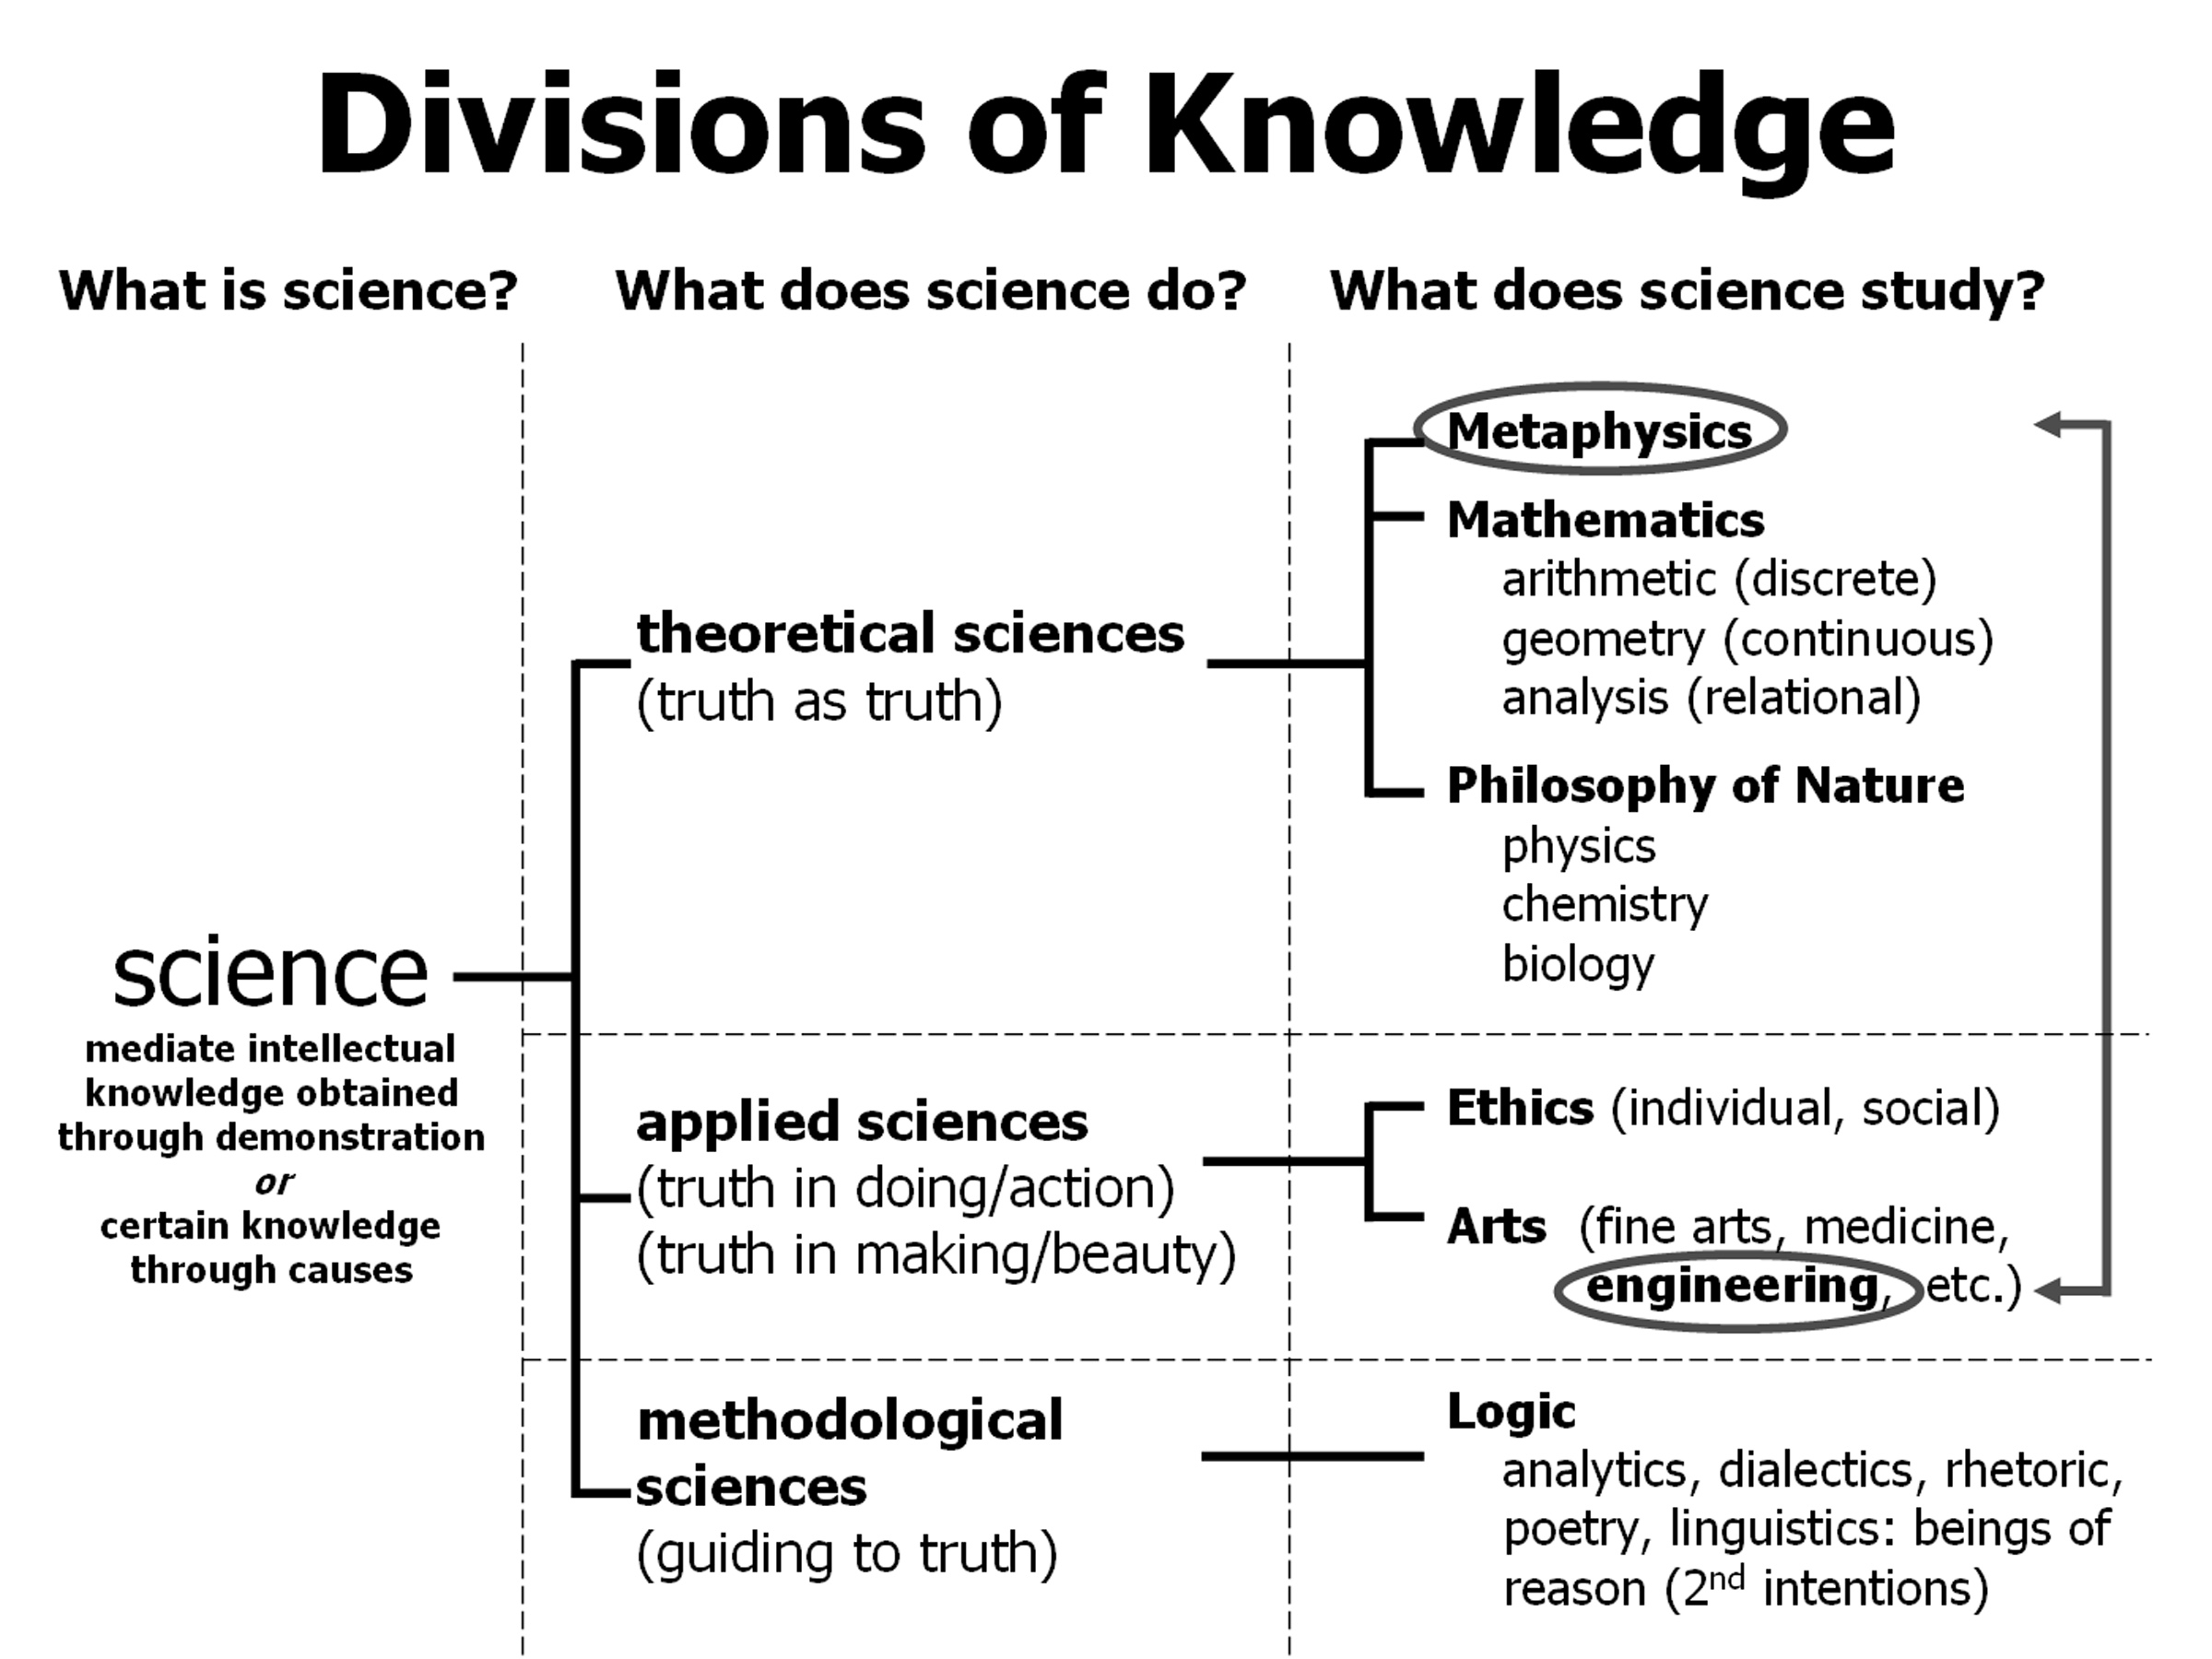
\includegraphics[scale=0.6]{sich_science_taxonomy.jpg}
\end{center}

All the particular (in the sense of ``individual'') sciences study different aspects of being. The question then becomes ``what are those \semph{fundamentally} distinguishing aspects or characteristics?''

\index{philosophy of nature}
Consider the speculative sciences. A discipline under the speculative sciences is the \sunder{philosophy of nature}, under which in turn can be distinguished the natural sciences:

\begin{itemize}
\item \sundertitle{Physics} studies matter in motion by modeling physical ``objects'' according to mathematically-formulated deterministic mechanisms;\footnote{Note for quantum mechanics one must be careful to distinguish the mathematical formalism employed to describe the behavior of objects that are highly affected by observation (measurement) from the natures of those objects. Epistemic limitations (in measurement) currently force us to employ statistical mathematical formalisms to describe observed quantum phenomena, but this in no way dictates the ontological status of those phenomena. The wave equation of an electron, for example, is derived from the observation of a huge population of electrons under specific conditions, but it does not follow that an electron is---by its nature---a wave: some wave-like behavior does not imply wave-like nature. An example might clarify this: the mathematical formalism known as a normal function describing the shape of the collection of balls that have fallen through a Galton board in no way implies the balls themselves---by their nature---are ``spread out'' in space or whose motions are \semph{random} (i.e., without cause). The Copenhagen Interpretation commits a gross error in logic and scientific procedure by concluding that what cannot be measured exactly does not occur exactly: an epistemic principle was converted into an ontological principle.}
\item \sundertitle{Chemistry} is concerned with the composition, structure, and properties of matter, as well as the changes matter undergoes during chemical reactions;
\item \sundertitle{Biology} studies living things---examining their structures, functions, growth, origin, distribution, and classification.
\end{itemize}

\index{mathematics}
\index{theology}
\index{logic}
\index{beings of reason}
\index{science!second intentions}
\sundertitle{Mathematics}, as a science, stands apart from the natural sciences because it studies being from which all properties (philosophically: accidents) abstracted except quantity---either discrete or continuous. In other words, mathematics studies being as quantified. \sunder{Metaphysics}, a science as well, stands above all---not just abstracting but \semph{separating} everything from being except those aspects shared by \semph{all} beings. \sundertitle{Theology} is a science: its subject matter is knowledge of God and Divine things obtained through philosophical reflection and argumentation. \sundertitle{Logic} studies beings of reason or second intentions. It is the science that seeks knowledge for its own sake and is productive of something for it organizes and guides reasoning to the truth. It is from this that we better see how levels of abstraction (from real beings to the object studied) distinguishes the sciences---yielding the subject matter of each of these disciplines.


\section[The Role of Abstraction]{The Role of Abstraction in Distinguishing the Particular Sciences\footnote{Many commentaries are available on the works of Aristotle and St. Thomas Aquinas that summarize the degrees of abstraction that distinguish the speculative sciences. See, for example, \citet[][pgs. 35--36]{maritain1959} and \citet[][pgs. 51--53]{velde2006}.}}

\index{abstraction!1st level (mathematics)}
\index{category (Aristotelian)}
\index{substance!primary}
\index{substance!secondary}
\index{being!changeable (ens mobile)}
(1) At the first level of abstraction, ``particular'' matter is left behind to focus upon ``general'' matter---where ``matter'' is understood in the logical sense. For example, the focus is not upon this red apple but upon the general notion of redness (physics) or the general notion of apples (biology) \semph{universally} applied to all particular objects studied. For the philosophy of nature, any particular red apple is termed a \semph{primary substance} while the universal ``apple'' is a \semph{secondary substance}; redness is an \semph{accident} (the Aristotelian category ``quality'') that can inhere in many different real objects. Another example is Socrates (primary substance) vs. human being (secondary substance). This first level of abstraction---generally applied to the philosophy of nature---resolves being in the sensible and the subject matter is \fword{ens mobile} (changeable being), while the individual natural sciences discriminate even further as noted above but worth repeating:

\begin{itemize}
\item Physics studies \semph{natural} material ``objects'' undergoing physical changes
\item Chemistry studies \semph{natural} material objects subject to electron-based interactions
\item Biology studies \semph{natural} living things
\end{itemize}

\index{artifact}
\index{nature (natural thing)}
\index{accidental unity}
``Natural''---or ``natures''---as the term is used here is not to be understood in the popular or ecological sense but as applied to those things in whom the principles for motion/change are immanent. \semph{Artifacts}, on the other hand, ultimately have their principles located externally to them. Stated philosophically, an acorn has the immanent capacity to actualize its nature into a mature oak tree.\footnote{For the distinction between natural things and artifacts: Aristotle, \btitle{Physics}, Book II, 192 b 9--18, 28. See also \citet{stump2006}.} A robot, which is technically termed an ``accidental unity,'' ultimately has its motion or change ``located'' (in the sense of ``explained'') as external to it: even a ``self-powered'' robot is not strictly that, for some external rational agent had to design the robot and impart upon it the ability to be ``self-powered.''

\index{essence}
Notice also the use of the word ``object'' particularly as applied to physics. When physics studies motion,\footnote{To be quite precise, physics does not study motion in the same sense that biology does not study life: neither “motion” nor “life” are, respectively, the objects of these sciences. \textit{Physics} studies material \textit{\textbf{things} in motion}; \textit{biology} studies \textit{living \textbf{things}} (or \textit{\textbf{things}} that were once living). “Things” here are understood as real, extra-mental existents accessible to (observable by) the five external senses or the senses enhanced through instrumentation. Neither “life” nor “motion” are \textit{per se} observable by the senses: we know “motion” and “life” exist, but only because we reflect upon the knowledge gained through the natural sciences, and that reflection properly belongs to the philosophy of nature. See, in particular, section IV paragraph 3 ahead.} it simplifies the things studied (termed an ``object'') in order to understand the motion, and then attempts to return to the fullness of reality by successively increasing the complexity of external influences. For example, a typical introductory Freshman-level physics course may pose the following problem: an \semph{object}, for which the final position is to be determined, is hurled into the air at such-and-such a speed in such-and-such a direction. It doesn't matter to physics whether that object is a marble, a howitzer round, or an elephant: physics does not focus on the essence (``whatness'') or nature of the object, and it doesn't need to\ldots nor can it. Once that basic level of motion is understood, one can then incorporate into the question other factors that will influence the motion: initial angular momentum, air resistance, expansion due to rapid heating, curvature of the earth, air currents, manufacturing flaws, etc., etc. In fact, given time, patience, and resources, one can proceed to any level of precision. \semph{But}, the full ontological import and essence of the ``object'' will never be captured by physics alone---let alone my mathematics.

\index{abstraction!2nd level (mathematics)}
(2) The second level of abstraction ``belongs'' to mathematics: all sensible aspects are left behind except the quantitative, and hence the beings studied are resolved not in the senses but in the imagination. Note that even highly abstract mathematical concepts (Lie groups, Fourier analysis, complex functions, etc.) must ultimately be reducible to discrete and continuous quantities abstracted from real objects. Mathematics is therefore the study of things that can be imagined and conceived without matter, not just the abstraction from the particular for the philosophy of nature and the individual natural sciences. The focus of mathematics is upon the first Aristotelian category of real being---quantity, again whether continuous (surfaces, volumes, etc.) or discrete (integers, countables, etc.) or relational (equations, inequalities, etc.).

\index{quantity!1st Aristotelian accident}
\index{being!extended in space (res extensa)}
Quantity, as the first accident of real being, is the basis for quality---the second accident of real being. For example, the average temperature of air in a room presupposes a non-point-like \fword{res extensa}---a thing spatially extended---and the ability to measure (quantify). Further, quality admits of degree; quantity does not. For example, no number (quantity) of kindergarteners adds up to the intelligence (quality) of Einstein.\footnote{It also makes for good jokes among scientists, e.g., 2 is equal to three for large values of two.} Finally, geometry, for example, is not concerned with the question whether a triangle (as imagined from some extra-mental object) is made of copper or of wood, but only with its absolute quantifiable nature, according to which it has three sides and three angles that add to 180 degrees in Euclidean (flat) space.

\index{abstraction!metaphysics (separation)}
\index{being!contingent}
(3) The final level of abstraction is actually ``separation'': all material aspects are left behind or ``separated'' from that which can exist without matter. Angels, for example, are purely immaterial beings and as such cannot in any way be imagined, for imagination requires an image---a picture---in the mind. Metaphysical terms such as unity, substance, soul, potency, causes, etc. exist without matter as well because such concepts apply to all extra-mental existents. Metaphysics, therefore, does not study being as changeable (philosophy of nature) or as quantifiable (mathematics) but being as being, and hence such being can only be resolved through concepts in the mind. As such, metaphysics is the study of the foundational principles of all beings---those aspects shared by \semph{all} contingent beings.

\index{ontology}
\index{metaphysics!transcendental}
In a strong sense, metaphysics is really at the heart of philosophy since it deals with the nature of reality in its widest throw. Metaphysics comprises two main areas or sub-disciplines: ontology and transcendental metaphysics. Ontology concerns itself with responding to the question ``what exists?'' while Transcendental Metaphysics concerns itself with the questions ``what is it for something to exist?'', ``are their different modes of existence?'', and ``if there are different modes of existence, what are the truth makers for these modes?'' More specifically, ontology attempts to formulate a complete list of all the fundamental categories of being, while transcendental metaphysics concerns itself with a fundamental understanding of essence, existence, nature, cause, etc., and the relationships between them, with the truth makers for modal claims, and with the transcendental attributes of being---attributes which apply to all beings simply as beings.

Consider the example of shoes. One can think of what is common to shoes, but one cannot draw it, i.e., quite literally one cannot imagine that commonality or universality known as ``shoeness'' shared among all shoes. As such, there is absolutely nothing which can be sensed---and hence measured---about ``shoeness.'' When one has an idea (not image!) of what is common to all shoes, of every shape, size, color, style, etc., one has grasped \sunder{conceptually} the form (formal cause---the ``whatness'')---the shoeness.

\section{Metaphysics: the Foundational Science}

\index{science!foundational (metaphysics)}
\index{science!fundamental (modern empirical)}
\index{science!particular}
So, metaphysics is the foundational philosophical discipline---quite literally \semph{the} foundational science. Whereas the modern empirical sciences (MESs) are the most fundamental form of knowledge we have because their objects are accessible to us through our senses, the MESs are neither the only form of knowledge nor the most important. All the particular (individual) sciences---including the productive sciences such as medicine and engineering and architecture---depend upon metaphysics for their ultimate presuppositions and basic principles. The particular sciences seek to understand their particular subject matters through the proximate ``ultimate'' causes within their particular domain. And, no science can prove its own proximately-considered first principles. There must be one foundational science (metaphysics) which seeks to understand all reality---all contingent beings---in terms of the universal properties of being as such.

\index{change!local motion}
\index{change!most general (natures)}
Consider the example of \semph{change}, and the species of change called ``local motion'' (translational, vibrational/oscillatory, and rotational/circular) through the following example. If one were to query a group of one hundred people chosen at random how many of them were seismologist that have modeled tectonic subduction zones, the expected response would be one, perhaps two of those people. If one then asked the same group how many had experienced an earthquake, the response might increase to about fifteen people. If one were then to ask the group how many know \semph{what} motion is, or at least experienced it, the hands of all the people in the group would be raised. This example highlights the difference between the narrowly- yet deeply-focused work of scientists, those who have had special experiences and hence knowledge, and the common knowledge shared by all healthy individuals.

\index{change!definition}
Motion (change of position of a material object as a function of time) for a physicist is relatively easy compared to the general notion of what motion is, for physics only asks ``how do things change/move?'' whereas the philosopher must ask ``\textit{\textbf{what} is} change in its widest throw?'' Motion for the philosopher is merely a species of change, for it is not merely a metaphor to assert, ``I was \semph{moved} by the beauty of my wife.'' There was a ``before'' when I was not moved, and then there was an ``after'' when my potential to be moved was actualized into reality---the reality of actually being in love. Hence, the most general definition (i.e., not the narrow physics-based definition) of motion is ``the reduction from potency to act, inasmuch as the object is in potency.''\footnote{According to Aristotle, motion must be defined as ``the act [entelechy] of that which exists in potency insofar as it is such'' (\fword{actus existentis in potentia secundum quod huiusmodi}), \btitle{Physics} 3.2, 201a27--29.} It was this general definition---based upon common experience accessible to all---that provide the foundation for physicists to do their good, mathematically-described work. Change had to be understood in its widest, most general throw before physics could narrow that understanding of change to study material objects in physical motion.

So, to revisit the three speculative sciences we can say

\begin{itemize}
\item \sundertitle{Physics} studies those things (material objects and physical phenomena) that have separate substantial (real, i.e., extra-mental) existence but are subject to change;
\item \sundertitle{Mathematics} studies those things free from change but which do not have separate substantial (real, i.e., extra-mental) existence: they exist only as distinguishable aspects of concrete realities. E.g., a tire's shape is a circle, the statistical distribution of students tests scores is described by a normal curve, etc.
\item \sundertitle{Metaphysics} studies those things that have separate substantial existence but are free from change---primarily the study of substances (as they are the primary mode of being): what aspects do all substances share?
\end{itemize}

\section{Quo Vadis, Engineering?}

Let us now focus our attention upon engineering as the applied science it is.

The metaphysician asks ``what is motion?'' The physicists asks, ``how do levers move under the influence of external forces?'' The engineer asks, how do I construct a structurally-sound bridge that will not move (within set parameters) under the influence of external forces?'' The differences between the questions asked, and hence the objects studied by these disciplines is profoundly different.

\index{science!speculative (theoretical)}
\index{science!applied (ethics, arts)}
The goal of the speculative (theoretical or ``pure'') sciences is to conform one's mind to reality. The goal of the applied sciences is to conform one's actions to reality, and by them we know (a) which actions conform to reality, (b) what we ought to do, and (c) how and why we should act.

\index{philosophy!moral}
\index{engineering!productive of artifacts}
In fact, one can only be successful in the applied sciences to the extent one is successful in the pure sciences. Ethics or moral philosophy answers the questions what should we do and why? The arts (including engineering as productive of ARTifacts) are---nay, must be---subordinate to ethics: one must first decide what one ought to do (which implies knowing why); then and only then may one enter into the details of how to do it. For example, knowing how to abort a child cannot trump knowing whether to do so. Another example is out ability, through science and technology, to detect weapons of mass destruction in Iran through remotes sensing. But no natural scientific, technological, or engineering discipline can then determine whether and what should be done about those weapons.

The applied sciences are subordinate to the speculative sciences as the speculative sciences are subordinate to the science that provides their principles---metaphysics. The knowledge obtained by the natural sciences must precede the application of the knowledge through engineering, and in that sense engineering is subordinate to the natural sciences as well.

So let's add engineering to our taxonomy in terms of the relationship it enjoys with the speculative sciences.

\begin{itemize}
\item \sundertitle{Metaphysics} is the study of being as being.
\item \index{science!modern empirical} The \sundertitle{modern empirical sciences} study the metrical properties (quantified observables) of changeable, material objects---objects particular to each natural science.
\item \index{philosophy of nature} The \sundertitle{philosophy of nature} stands between these two disciplines as the study of all changeable beings---of the general properties of all real (extra-mental, substantial and accidental) existents.
\item The \sundertitle{engineering disciplines} apply the knowledge gained from the natural sciences to achieve practical ends---to the making of artificial things (artifacts---\semph{not} natures).
\item \index{philosophy of science!methodological epistemology} The \sundertitle{philosophy of science} studies systems of reasoning (methodological epistemology) of natural things.
\end{itemize}

So, we see metaphysics is ultimately connected to engineering because it studies the first causes and principles of all beings---including those things studied by the modern empirical sciences and engineering.

However, the modern empirical sciences are ``closer'' to metaphysics because

\begin{enumerate}
\item they are speculative (theoretical) in the same way metaphysics is
\item the modern empirical sciences provide real-world knowledge for metaphysics to reflection upon
metaphysics, through natural philosophy, provides the modern empirical sciences with foundational (proximate ``first'') principles
\end{enumerate}

In contrast, engineering is ``located'' further from metaphysics because

\begin{enumerate}
\item it is applied knowledge (productive of artifacts) rather than speculative
\item it depends upon the MESs to provide knowledge of the real world
\item it provides metaphysics no direct substantive knowledge of the real world upon which to reflect
\item metaphysics---through the philosophy of nature and the modern empirical sciences---provides engineering with foundational principles
\item it is subject to the constraints of the practical sciences (e.g., ethics)
\end{enumerate}

\index{technology!techne (artifact)}
Productive reasoning involves having what one might be tempted to call ``creative'' ideas. In fact, productive ideas are based upon some understanding of the forms that matter can take, supplemented by imaginative thinking about such details as sizes, shapes, and configurations. Scientific knowledge can indeed be applied productively: scientific knowledge, through \semph{technology} (= scientific know-how), provides us with the skills and power to produce things.

But the philosophical reflection that improves our common-sense grasp of the physical world in which we live gives us neither the skill nor the power to produce anything. Philosophy bakes no cakes and builds no bridges. So, is it ``useless'' in the Marxist sense? No. Echoing more strongly a previous point, philosophical knowledge lays the foundations of our thinking and can be ``used'' to direct lives and manage societies: philosophy animates for the sake of doing---not directly for the sake of making, which is why ``making'' must be subordinate to ``doing.''

\index{artifact!art imitates nature (Aristotle)}
\index{nature!natural thing!art imitates nature (Aristotle)}
There is also an analogical connection of metaphysics to engineering insofar as metaphysicians can draw analogies from the way things are made and function to make inferences about those things that cannot change. This reflects Aristotle's crucially-important principle: \sbf{art(ifact) imitates nature}, and not the other way around.

\index{telos}
\index{reasoning!productive}
\index{reasoning!speculative}
To anticipate a possible criticism: some may point to the Ancient Egyptians as an example of those who did not know physics yet built the pyramids and statues, or Ancient Romans who also did not know physics yet built roads and aqueducts, so that engineering \semph{can} precede science. Well, not really. In the order of knowing, one must first understand---even if inchoately---that rocks fall when released and crumble when too high a load is imposed. Such knowledge must precede the application of that knowledge. To build something is not to ``do'' engineering, in the same sense that technology cannot be equated to science. To categorize the smart folks of those times as ``scientists'' or ``engineers'' is actually incorrect if ``science'' and ``engineering'' are understood to be what they are to us moderns, unless one does so analogously. This is not to suggest that engineering does not inform the natural sciences---it does, quite significantly. However, there is \semph{no reason whatsoever} for engineering to explore physical reality other than to \semph{make} something---an artifact. If engineering's goal is simply to know, then it is no longer engineering but physics or chemistry or whatever natural science. Engineering's \fword{telos}---its end or goal---for studying reality is to make something, not to know simply for the sake of knowing.

\section[A Case Study]{A Case Study in the Failure to Properly Distinguish: Intelligent Design}

\index{reductionism!mechanistic}
Needless to say, a mistake often made is to forget (or neglect\ldots perhaps even intentionally) this principle, and hence to fall into one of the most common errors: the fallacy that nature imitates art(ifact)---the ``mechanistic'' reductionist error shared by Intelligent Design and DarwinISM. Consider the following claims:

\begin{enumerate}
\item \index{Behe, Michael} Intelligent Design proponent Michael Behe: ``Modern science reveals the \sbf{cell is a} sophisticated, automated, nanoscale \sbf{factory}.''\citep{beheinterview} [bold-face emphasis added]
\item \index{Alberts, Bruce} Darwinist Bruce Alberts: ``The entire \sbf{cell can be viewed as a factory} that contains an elaborate network of interlocking assembly lines, each of which is composed of a set of large protein machines\ldots Why do we call the large protein assemblies that underlie cell function protein \emph{machines}? Precisely because, like machines invented by humans to deal efficiently with the macroscopic world, these protein assemblies contain highly coordinated moving parts '' \citep{balberts}. [bold-face emphasis added]
\end{enumerate}

This is terribly muddled thinking that flips reality on its head, and Behe's claim is all the worse because it asserts, while Alberts at least qualifies his claim with ``can be viewed as.''

\index{bacterial flagellum}
\index{cell!natural thing}
\index{motor!art}
The nature or essence of a bacterial flagellum, for example, might be considered from the \semph{artificial} (note the root ``artifact'') perspective as that of a motor (a machine---an accidental unity) \semph{but only if considered in isolation from the cell}.\footnote{The point of the flagellum ``considered \semph{in isolation} from the cell'' is also important because it highlights another form of reductionism in Behe's thinking. To study most of the aspects of a bacterial flagellum (and certainly to study the components of the flagellum and their properties), the cell must be destroyed (Nature must not only be interrogated but tortured as well--harkening back to Francis Bacon's \fword{novus ordo seclorum} control over Nature), i.e., the flagellum is studied in a pathological state removed from the \semph{substance} known as the bacterial cell.} However, it is not Behe's empirical observations that indicate to him the flagellum is a motor: he drew upon empirical observations to reason to the intelligible aspect of that thing known through the universal concept of ``motor,'' i.e., it required an immaterial nous (intelligent agent) to ``know'' the immaterial intelligible aspect of that particular biological system.

\index{per accidens}
\index{telos}
\index{concept!universal}
\index{functionality}
Ric Machuga pointedly explains Behe and Dembski's misguided attempt to quantify an object's form (formal cause or specificity) and \textit{telos} (final cause or function) by providing the example of pincers: neither mathematics nor the natural sciences can tell us what the tweezers in my hand, the pliers in my tool box, the bigger pliers in my plumber's tool box, the pincers of a lobster's claw, the forceps of a surgeon, the mandibles of a bull ant, the jaw of a human being, or a fireman's ``jaws of life'' are. And yet, any intelligent agent can explain that all these examples are understood by the \semph{universal (i.e., not concrete and hence immaterial) concept} of a compound lever. There is \semph{nothing} about \semph{what} a compound lever \semph{is} that physics or mechanical engineering can tell anyone---apart from \semph{how} one works: the moment arms involved, the pressure applied at the point of contact, the position of the fulcrum, etc. Natural philosophy, on the other hand, not only permits one to ``see'' the \fword{quiddity} (``whatness'') of the object, but in the list provided it can distinguish between the three examples of \fword{per se} unities and the five examples of \fword{per accidens} unities. Machuga correctly concludes:

\begin{quote}
The only thing all pincers have in common is an intended purpose, design, of function---in short, a form. While quantifiable shapes can be the embodiment of forms, no form can be reduced to a quantifiable shape \cite[pg.~162]{machuga}.\footnote{Note for pedagogical reasons Machuga uses the term ``shape'' to capture all nine accidents (Aristotelian categories) of real being: `` `Shape,' as we are using the term, refers to the totality of a thing's physically quantifiable properties, i.e., its physical shape and size, height, weight, chemical composition, etc., in its most complete description\ldots It is what the sciences study.'' (pg. 27)}
\end{quote}

\index{design}
\index{Intelligent Design}
While provocative, it is nonetheless true: Intelligent Design is neither a science nor engineering. Intelligent Design is weak philosophizing imposed upon scientific findings, which the following example will help to clarify. Physicists inferred the existence of a material object---the neutrino---from physical observables, i.e. from the apparent violation of conservation of energy and angular momentum in beta decay processes. Intelligent Design theorists attempt to infer the existence of ``design'' and hence a designer. But this, of course, begs the question: is design the same ontological kind of thing as a neutrino? No, for unless one is a materialist or other such reductionist (which is a hidden irony of Intelligent Design), design is a very different kind of thing than a neutrino.  This, in turn, then demands a very different \semph{kind of science} to study design---not a natural science, but a philosophical science.

This confusion arises precisely because Intelligent Design fails to properly distinguish their subject matter, i.e., they haven't asked the question: ``is a neutrino the same \semph{kind} of thing as `design'?'' As a result of Intelligent Design ontologically ``flatlanding'' (or ``domesticating'') design down to the level of material objects, it then attempts to ``measure'' and ``quantify'' formal and final causality. And, it also unnecessarily pits efficient causality against final causality.

\index{abstraction}
Design is an abstraction based on sensory observations, and philosophical arguments are needed to infer to its existence, just like philosophical arguments are used to support the efficacy of scientific method. A neutrino, on the other hand, is not an abstraction: it is a real, substantive, extra-mental material object. ``Design'' is a combination of formal causality (whatness) and final causality (function or ``for what'') that partly explains the existence of artifacts---\semph{not} natural things.

\index{functionality!mathematically ambiguous}
\index{mathematics}
\textit{Functionality} or ``irreducible complexity''\footnote{Behe defines an irreducibly complex system as one “composed of several well-matched, interacting parts that contribute to the basic function, wherein the removal of any one of the parts causes the system to effectively cease functioning.” \citep[][pg. 39]{behe2006}} per Michael Behe is, in fact, mathematically ambiguous, and in no way can it be measured---despite uninformed protestations to the contrary. Functionality implies a \textit{telos}---a “for whatness” or final cause, which is neither a subject matter (formal object) nor material object studied by any of the modern empirical sciences.  To repeat Machuga's point above, if one considers a pair of pliers, a nut cracker, an insect's mandibles, and a lobster claw, we have one and the same \textit{functionality} applied to different situations: to hold tight and possibly crush an object. Yet, their complexities vary exceedingly widely. Which of these objects has more ``\textit{functionally} specified information''? Stephen Meyers explicitly claims ``Dembski's theory\ldots applies to any system that has large amounts of such functional information.''\cite[pg.~372]{sigcell} Large amounts of functional information? Are jaws-of-life ``more'' \textit{functional} than a pair of household pliers, or are they simply more \textit{complex}?  How exactly is one to measure---literally to quantify by means of a metric---the differences in function between the physical examples above? Again, one cannot mathematically distinguish functions: the function is the same for all the examples above (and many more), while their mathematically-describable complexities (through the correlation of sensory-accessible properties into mathematical formalisms) vary widely.  Complexity and information are quantifiable, while functionality and essence (meaning) are not.

\index{specified complexity!mathematically ambiguous}
Similarly, what a thing is---or, to employ William Dembski's term, its ``specified complexity''\footnote{For a fair summary, including definitions, mathematical treatment, criticisms, and references see “Specified Complexity” (http://en.wikipedia.org/wiki/Specified\_complexity\#cite\_note--8)}---is also mathematically ambiguous, and Intelligent Design actually fails to properly distinguish ``information'' (which is measurable) from ``meaning'' (which is not measurable).  Intelligent Design literally conflates the two. To be ``specified'' is to be a \textit{specific} thing, to be an actualized existent---a \textit{substance} that is \textit{understood} or intelligible or whose whatness is known. In other words, it is the formal cause of a thing Dembski is attempting---and failing---to quantify.  If I (1) employ smoke to sky--write the Ukrainian word \sbf{\foreignlanguage{russian}{ЧЕРВОНЕ}} in all--caps, bold--faced, with letters each 100 meters tall, and if I print on paper the English word ``red'' in small--case 8--point font size, these two words have (gender signification notwithstanding in Ukrainian) \semph{precisely the same meaning}. Yet, the information content required to represent the physical aspects of these two words in a computer's memory would be very different.  Nonetheless, Dembski claims (which the scientific correctly community rejects, even as it vaguely understands): ``if there is a way to detect design, specified complexity is it.'' \citep[][pg. 19]{dembskinfl}

\index{nature!natural thing}
\index{artifact}
Finally, Intelligent Design presupposes that living organisms are artifacts with externally-imposed functionality and form. These organisms are then implicitly viewed as passive, mechanistic receptors of an occasionalist designer's tinkering. As such, it fails to consider even clear Biblical evidence that God creates not individual things but natures---natures which actualize, through their immanent capacities or powers---to perfections (understood philosophically) like the earlier example of the acorn growing into a mature oak tree: God doesn't ``make'' oak trees (note the inherent engineering reductionism of a natural thing to an artifact), acorns ``make'' oak trees. Consider Genesis 1:11--12, 20, 24 where the \semph{\sunder{earth} brought forth}\ldots the \semph{\sunder{seas} brought forth}. Intelligent Design demotes God's timeless, existence-sustaining creative act to some ``thing'' accessible to natural scientific inquiry.

\index{God!domestication of}
\index{God!cause among causes}
\index{God!being among beings}
At the end of the day, Intelligent Design is an attempt to study miracles through natural scientific means. As such, it tries in vain to ``domesticate'' God down to the level of efficient causes in the real world because its proponents want to ``detect'' or ``infer'' His existence \semph{directly} through natural scientific means\ldots as the ugly step-sister of the even uglier step-son of atheists trying to disprove God through the natural sciences. Intelligent Design proponents want to ``infer'' God's direct actions from material entities by understanding Him as acting directly in biological organisms, which is another manifestation of the error of occassionalism.  In other words, God is reduced to another causes among causes, and hence another being among beings.

As St. Paul instructs us, because we are by nature rational animals, we are capable of knowing ``God's eternal power and divinity'' from ``the things He has made'' (Romans 1:19--20), i.e., by the light of human reason alone:

\begin{quote}
\semph{For what can be known about God is evident to [the wicked], because God made it \sbf{evident} to them. Ever since the creation of the world, His \sbf{invisible} attributes of eternal power and divinity have been able to be \sbf{understood and perceived} in what He has made}.'' (emphasis added)
\end{quote}

The knowledge presupposed by St. Paul in this passage cannot possibly be of beautiful galactic nebula, bacterial flagella, cosmic fine-tuning, or engineering system analysis of cell processes---there were no modern empirical sciences at that time! Rather, this knowledge must be grounded in pre-scientific common experience and philosophical reflection animated by the presuppositions and intellectual habits whose origin is in a Christian world view.

\index{design}
\index{reductionism}
\index{Intelligent Design}
Permit me to be provocative again: one would have to be out of one's mind to deny design in the universe. But, the reductionist view of ``design'' proffered by Intelligent Design proponents and ``design'' as understood by critically-thinking philosophers are two very different things. Reason alone and independently (as well as faith alone or independently) can lead us to the ``existence'' of the Creator, but the path is in and through philosophy---not in the natural sciences or engineering. No amount of empirical data can defeat a metaphysical proof. Clearly, empirical data, scientific theories, and engineering expertise \semph{inform} metaphysical reasoning, such reasoning is impervious to empirical falsification---similar to a mathematical theorem not being falsifiable by any empirical data.

\index{philosophical naturalism}
\index{scientism}
\index{Intelligent Design}
No empirical data or scientific theory exist in a vacuum: there is no ``preferred'' metaphysical interpretation attached. Yet, interpretations there must be. Whether implicitly or explicitly, secularist scientists embrace the pseudo-philosophy of ``philosophical'' naturalism and materialism as animated by scientism. To counter this, the Intelligent Design movement cannot hope to exclusively misappropriate science\ldots or especially to find a ``new home'' in engineering: it must adopt a realist philosophy of nature. That is where the real battle for the mind is fought---not in or through the natural sciences. What this implies, of course, is that Intelligent Design proponents must face some deep soul-searching to realize Intelligent Design indeed does not belong in the biology classroom any more than DarwinISM does. That is the only way the Intelligent Design movement will reclaim the high ground, and in my humble opinion only then will it be unstoppable.

\index{science!subject matter}
The failure to distinguish the proper roles and subject matters studied by the natural sciences, metaphysics, and engineering will only lead to confusion\ldots of which Intelligent Design and DarwinISM are only two unfortunate examples.\footnote{See \citet[][pg. 372]{sigcell} for an example.}. However, when these disciplines are respected and their differences celebrated (a tuba would sound ugly usurping the part of a piccolo), i.e., if they are permitted to operate as a symphony productive of truth---with the particular science as the individual instruments, metaphysics as the conductor, and God as the composer---the music would, indeed, be Divinely beautiful.

\eandmbibliography{SichLibrary}
